\documentclass[a4paper,12pt]{extarticle}
\usepackage[utf8x]{inputenc}
\usepackage[T1,T2A]{fontenc}
\usepackage[russian]{babel}
\usepackage{hyperref}
\usepackage{indentfirst}
\usepackage{listings}
\usepackage{color}
\usepackage{xcolor}
\usepackage{here}
\usepackage{array}
\usepackage{multirow}
\usepackage{graphicx}
\usepackage{amsmath}

\hypersetup{
    colorlinks = false,
    linkbordercolor = {white}
}

\definecolor{string}{HTML}{B40000} % цвет строк в коде
\definecolor{comment}{HTML}{008000} % цвет комментариев в коде
\definecolor{keyword}{HTML}{1A00FF} % цвет ключевых слов в коде
\definecolor{morecomment}{HTML}{8000FF} % цвет include и других элементов в коде
\definecolor{сaptiontext}{HTML}{FFFFFF} % цвет текста заголовка в коде
\definecolor{сaptionbk}{HTML}{999999} % цвет фона заголовка в коде
\definecolor{bk}{HTML}{FFFFFF} % цвет фона в коде
\definecolor{frame}{HTML}{999999} % цвет рамки в коде
\definecolor{brackets}{HTML}{B40000} % цвет скобок в коде

\usepackage{caption}
\renewcommand{\lstlistingname}{Программа} % заголовок листингов кода

\bibliographystyle{ugost2008ls}

\usepackage{listings}
\lstset{ %
	extendedchars=\true,
	keepspaces=true,
	language=Python,						% choose the language of the code
	% Цвета
	keywordstyle=\color{keyword}\ttfamily\bfseries,
	%stringstyle=\color{string}\ttfamily,
	stringstyle=\ttfamily\color{red!50!brown},
	commentstyle=\color{comment}\ttfamily\itshape,
	morecomment=[l][\color{morecomment}]{\#},
	basicstyle=\footnotesize,		% the size of the fonts that are used for the code
	numbers=left,					% where to put the line-numbers
	numberstyle=\footnotesize,		% the size of the fonts that are used for the line-numbers
	stepnumber=1,					% the step between two line-numbers. If it is 1 each line will be numbered
	numbersep=5pt,					% how far the line-numbers are from the code
	backgroundcolor=\color{white},	% choose the background color. You must add \usepackage{color}
	showspaces=false				% show spaces adding particular underscores
	keywordstyle=color{blue}\bfseries, 
	showstringspaces=false,			% underline spaces within strings
	showtabs=false,					% show tabs within strings adding particular underscores
	frame=single,          		% adds a frame around the code
	tabsize=2,						% sets default tabsize to 2 spaces
	captionpos=t,					% sets the caption-position to top
	breaklines=true,				% sets automatic line breaking
	breakatwhitespace=false,		% sets if automatic breaks should only happen at whitespace
	escapeinside={\%*}{*)},			% if you want to add a comment within your code
	postbreak=\raisebox{0ex}[0ex][0ex]{\ensuremath{\color{red}\hookrightarrow\space}},
	texcl=true,
	inputpath=listings,                     % директория с листингами
}

\usepackage[left=2cm,right=2cm,
top=2cm,bottom=2cm,bindingoffset=0cm]{geometry}

%% Нумерация картинок по секциям
\usepackage{chngcntr}
\counterwithin{figure}{section}
\counterwithin{table}{section}

%%Точки нумерации заголовков
\usepackage{titlesec}
\titlelabel{\thetitle.\quad}
\usepackage[dotinlabels]{titletoc}

%% Оформления подписи рисунка
\addto\captionsrussian{\renewcommand{\figurename}{Рисунок}}
\captionsetup[figure]{labelsep = period}

%% Подпись таблицы
\DeclareCaptionFormat{hfillstart}{\hfill#1#2#3\par}
\captionsetup[table]{format=hfillstart,labelsep=newline,justification=centering,skip=-10pt,textfont=bf}

%% Путь к каталогу с рисунками
\graphicspath{{fig/}}

\begin{document}	% начало документа

% Титульная страница
%\begin{titlepage}	% начало титульной страницы

	\begin{center}		% выравнивание по центру

		Санкт-Петербургский Национально Исследовательский Университет\\
		информационных технологий, механики и оптики \\
		Кафедра систем управления и информатики\\[3cm]
		% название института, затем отступ 6см
		
		\huge \textbf{РЕФЕРАТ}\\[0.5cm]
		\large Электромеханические системы\\[0.1cm]
		\large Система автоматического управления квадракоптера Parrot ARDrone 2.0\\[2cm]

	\end{center}


	\begin{flushright} % выравнивание по правому краю
%		\begin{minipage}{0.5\textwidth} % врезка в половину ширины текста
%			\begin{flushleft} % выровнять её содержимое по левому краю

				\large Выполнили студенты группы P3335\\
				\large А.М. Зенкин\\[0.5cm]
				\large К.В. Карпов\\[0.5cm]
				
				\large Принял  к.т.н., доцент кафедры СУиР\\
				\sign[4cm]\large  М.С. Чежин\\
				\large Оценка: \sign\\
				«\underline{\hspace{0.7cm}}» \underline{\hspace{2cm}} \the\year г.

%			\end{flushleft}
%		\end{minipage}
	\end{flushright}
	
	\vfill % заполнить всё доступное ниже пространство

	\begin{center}
	\large Санкт-Петербург\\
	\large \the\year % вывести дату
	\end{center} % закончить выравнивание по центру

\thispagestyle{empty} % не нумеровать страницу
%\end{titlepage} % конец титульной страницы
\newpage


% Содержание
% Содержание
\renewcommand\contentsname{\centerline{Содержание}}
\tableofcontents
\thispagestyle{fancy}
\newpage




\section{Цель работы}
Ознакомление с методами взаимного перехода между моделями вход-выход и вход-состояние-выход, а также с каноническими формами представления моделей вход-состояние-выход.


\section{Варианты параметров}
$n = 3$, $a_0 = 7$, $a_1 = 5$, $a_2 = 2$, $b_0 = 10$, $b_1 = 3$, $b_2 = 1.5$\\

$n = 2$,  $A = \begin{bmatrix}
				0.5 & -10\\
				1 & -2
				\end{bmatrix}$, $B = \begin{bmatrix}
									0\\
									1
									\end{bmatrix}$, $C^T = \begin{bmatrix}
															3\\
															1
															\end{bmatrix}$\\			
													
$M = \begin{bmatrix}
				4 & 0\\
				-2 & 0.5
				\end{bmatrix}$															


\section{Ход выполнения работы}

\subsection{Переход от модели вход-выход к модели вход-состояние-выход.}

\subsubsection{Математические вычисления:}
\paragraph{Определение передаточной функции:}
\begin{equation}
	\begin{split}	
&\dddot{y} + 2\ddot{y} + 5\dot{y} + 7y = 1.5\ddot{u} + 3\dot{u} + 10u;\\
&s^3y + 2s^2y + 5sy = 1.5s^2u + 3su + 10u;\\
&y=\frac{1.5s^2+3s+10}{s^3+2s^2+5s+7}u;\\
&W(s)=\frac{1.5s^2+3s+10}{s^3+2s^2+5s+7};\\
	\end{split}
\end{equation}
\paragraph{Построение модели ВСВ в к.у.ф.:}
\begin{equation}
	\begin{split}	
A = \begin{bmatrix}
				0 & 1 & 0\\
				0 & 0 & 1\\
				-7 & -5 & -2
				\end{bmatrix}; B = \begin{bmatrix}
				0\\
				0\\
				1
				\end{bmatrix}; C = \begin{bmatrix}
				10 & 3 & 1.5
				\end{bmatrix};\\
	\end{split}
\end{equation}
\paragraph{Построение модели ВСВ в к.н.ф.:}
\begin{equation}
	\begin{split}	
A = \begin{bmatrix}
				0 & 0 & -7\\
				1 & 0 & -5\\
				0 & 1 & -2
				\end{bmatrix}; B = \begin{bmatrix}
				10\\
				3\\
				1.5
				\end{bmatrix}; C = \begin{bmatrix}
				0 & 0 & 1
				\end{bmatrix};\\
	\end{split}
\end{equation}

\subsubsection{Моделирование моделей вход-выход, вход-состояние-выход в канонической управляемой форме и вход-состояние-выход в канонической наблюдаемой форме при ступенчатом единичном входном воздействии и нулевых начальных условиях:}

\begin{figure}[H]
	\begin{center}
		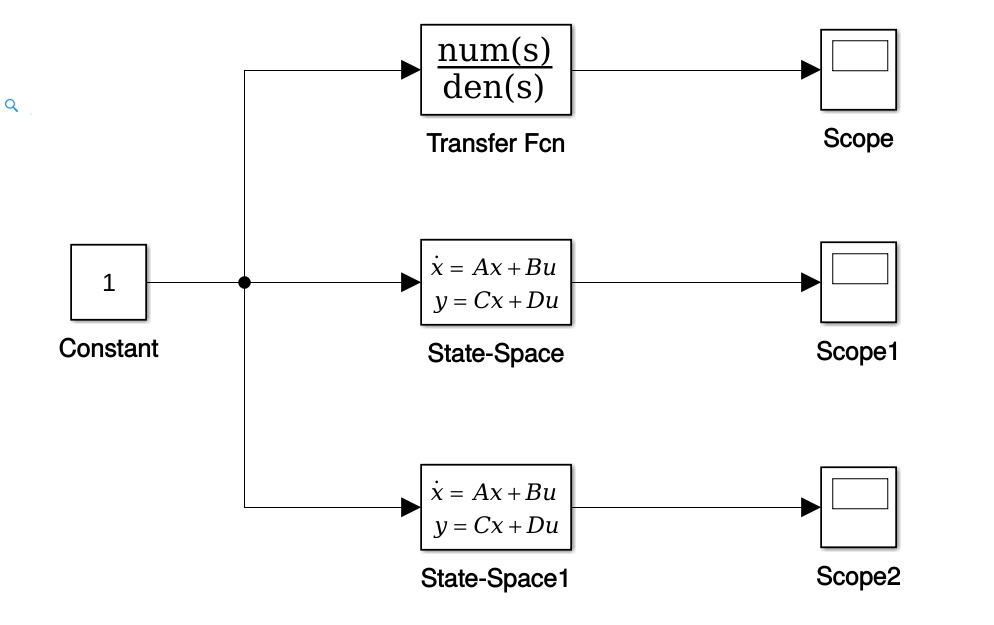
\includegraphics[scale=0.25]{IOtoISO}
		\caption{схема моделирования $u(t) = 1$} 
		\label{pic:pic_1} % название для ссылок внутри кода
	\end{center}
\end{figure}

\begin{figure}[H]
	\begin{center}
		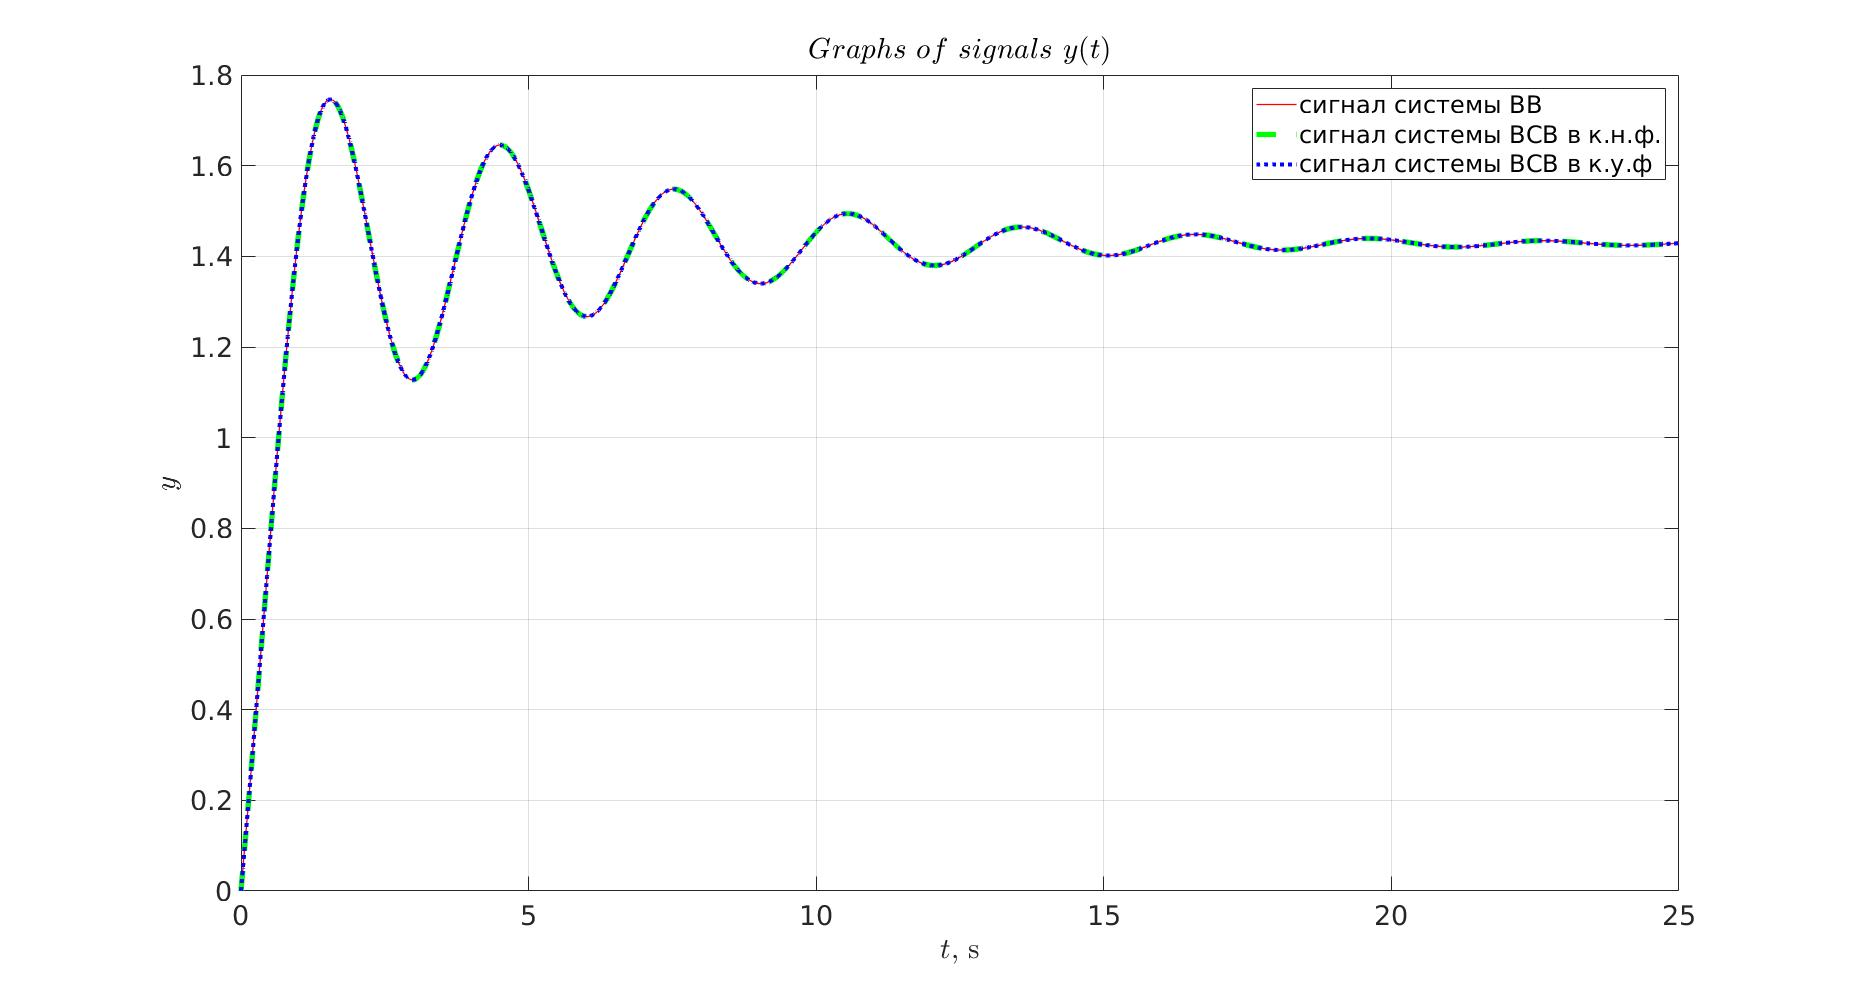
\includegraphics[scale=0.28]{part1}
		\caption{графики моделирования системы} 
		\label{pic:pic_2} % название для ссылок внутри кода
	\end{center}
\end{figure}

\subsection{Переход от модели вход-состояние-выход к модели вход-выход.}
\subsubsection{Математические вычисления:}
\paragraph{Определение передаточной функции:}
\begin{equation}
	\begin{split}	
	&A = \begin{bmatrix}
				0.5 & -10\\
				1 & -2
				\end{bmatrix}, B = \begin{bmatrix}
									0\\
									1
									\end{bmatrix}, C^T = \begin{bmatrix}
															3\\
															1
															\end{bmatrix};\\
&W(s)=C(SI-A)^{-1}B;\\
&W(s)=\begin{bmatrix}
				3 & 1\\
				\end{bmatrix}\Biggl(\begin{bmatrix}
				s & 0\\
				0 & s
				\end{bmatrix} - \begin{bmatrix}
				0.5 & -10\\
				1 & -2
				\end{bmatrix}\Biggr)^{-1}\begin{bmatrix}
				0\\
				1
				\end{bmatrix};\\
&W(s)=\begin{bmatrix}
3 & 1\\
\end{bmatrix}\begin{bmatrix}
\frac{s+2}{s^2+1.5s+9} & \frac{-10}{s^2+1.5s+9}\\
\frac{1}{s^2+1.5s+9} & \frac{s-0.5}{s^2+1.5s+9}\\
\end{bmatrix}\begin{bmatrix}
0\\
1\\
\end{bmatrix};\\
&W(s)=\frac{s-30.5}{s^2+1.5+9};\\
	\end{split}
\end{equation}

\paragraph{Модель вход-выход:}

\begin{equation}
	\begin{split}	
&\ddot{y} + 1.5\dot{y} + 9y = \dot{u} - 30.5u;\\
	\end{split}
\end{equation}

\paragraph{Модель вход-состояние-выход в к.у.ф.:}
\begin{equation}
	\begin{split}
		&A=\begin{bmatrix}
		0 & 1\\
		-9 & -1.5\\
		\end{bmatrix} B=\begin{bmatrix}
		0\\
		1\\
		\end{bmatrix} C=\begin{bmatrix}
		-30.5 & 1\\
		\end{bmatrix}\\
	\end{split}
\end{equation}
\paragraph{Модель вход-состояние-выход в к.н.ф.:}
\begin{equation}
	\begin{split}
		&A=\begin{bmatrix}
		0 & -9\\
		1 & -1.5\\
		\end{bmatrix} B=\begin{bmatrix}
		-30.5\\
		1\\
		\end{bmatrix} C=\begin{bmatrix}
		0 & 1\\
		\end{bmatrix}\\
	\end{split}
\end{equation}
\subsubsection{Моделирование исходной модели и полученных моделей вход-выход, вход-состояние-выход в канонической управляемой форме и вход-состояние-выход в канонической наблюдаемой форме, при ступенчатом единичном входном воздействии и нулевых начальных условиях:}

\begin{figure}[H]
	\begin{center}
		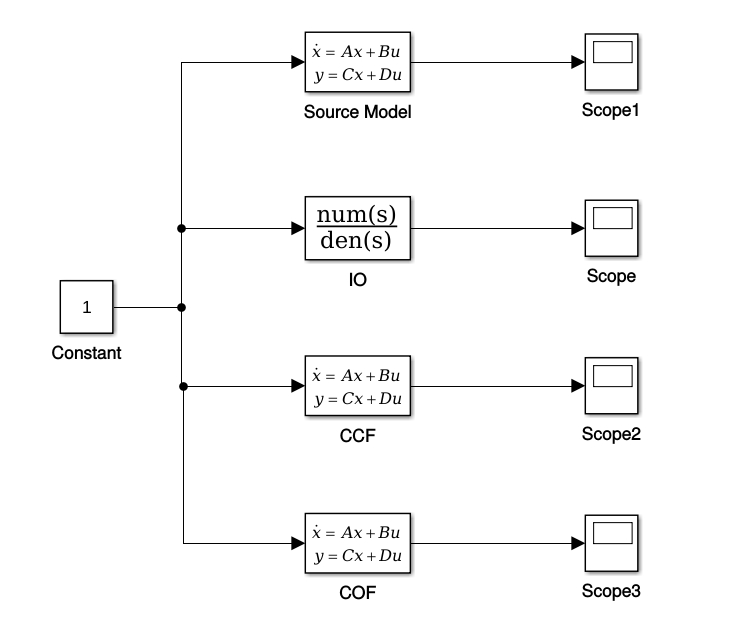
\includegraphics[scale=0.3]{ISOtoIO}
		\caption{схема моделирования $u(t) = 1$} 
		\label{pic:pic_3} % название для ссылок внутри кода
	\end{center}
\end{figure}

\begin{figure}[H]
	\begin{center}
		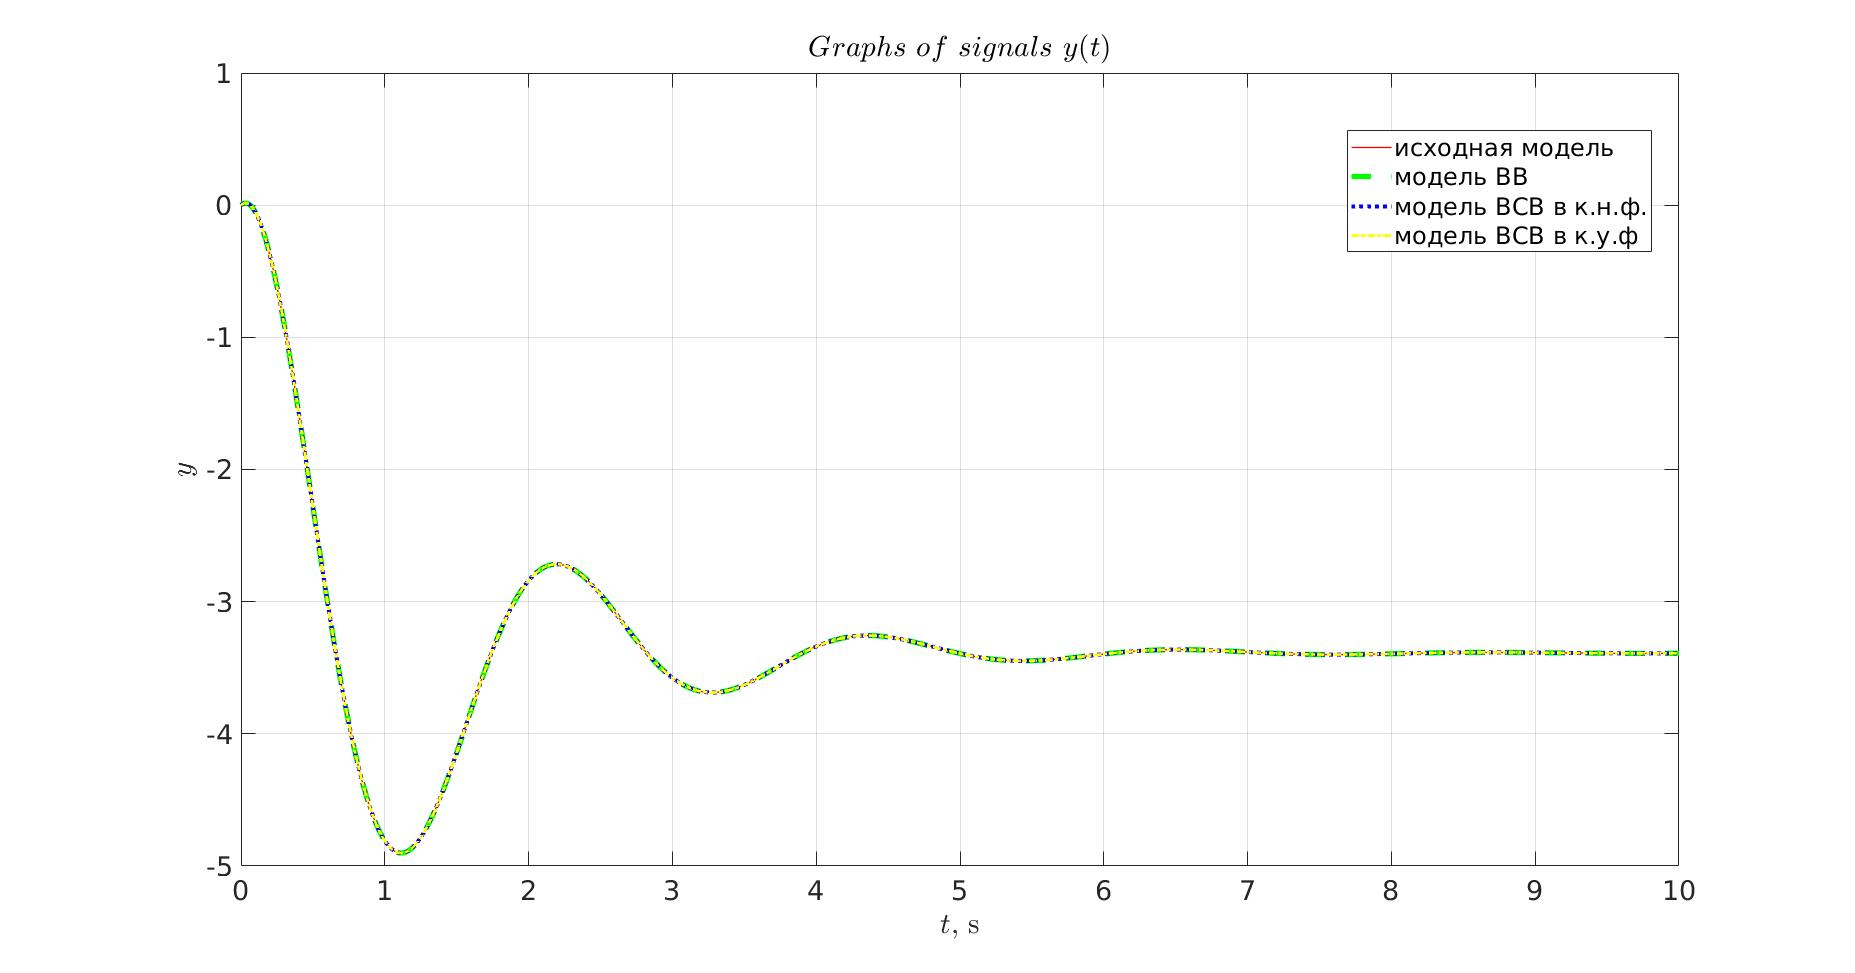
\includegraphics[scale=0.28]{part2}
		\caption{графики моделирования системы} 
		\label{pic:pic_4} % название для ссылок внутри кода
	\end{center}
\end{figure}

\subsubsection{Рассчёт матрицы преобразования исходной модели к каноническим формам:}

\paragraph{Для модели ВСВ в к.у.ф.:}

\begin{equation}
	\begin{split}	
		&M=N_y\Hat{N_y}^{-1}, N_y=[B\vdots AB], \Hat{N_y}=[\Hat{B}\vdots \Hat{A}\Hat{B}];\\
		&N_y=\begin{bmatrix}
			0 & -10\\
			1 & -2\\
		\end{bmatrix}, \Hat{N_y}=\begin{bmatrix}
					   		0 & 1\\
					   		1 & -1.5\\
					   \end{bmatrix}, \Hat{N_y}^{-1}=\begin{bmatrix}
					   						1.5 & 1\\
					   						1 & 0\\
					   				  \end{bmatrix};\\
		&M=\begin{bmatrix}
			-10 & 0\\
			-0.5 & 1\\
		\end{bmatrix};\\
	\end{split}
\end{equation}

\paragraph{Для модели ВСВ в к.н.ф.:}

\begin{equation}
	\begin{split}	
		&M=N_y\Hat{N_y}^{-1}, N_y=[B\vdots AB], \Hat{N_y}=[\Hat{B}\vdots \Hat{A}\Hat{B}];\\
		&N_y=\begin{bmatrix}
			0 & -10\\
			1 & -2\\
		\end{bmatrix}, \Hat{N_y}=\begin{bmatrix}
					   		-30.5 & -9\\
					   		1 & -32\\
					   \end{bmatrix}, \Hat{N_y}^{-1}=\begin{bmatrix}
					   						-\frac{32}{985} & \frac{9}{985}\\
					   						-\frac{1}{985} & -\frac{61}{1970}\\
					   				  \end{bmatrix};\\
		&M=\begin{bmatrix}
			\frac{2}{197} & \frac{61}{197}\\
			-\frac{6}{197} & \frac{14}{197}\\
		\end{bmatrix};\\
	\end{split}
\end{equation}

\newpage

\subsection{Замена базиса в пространстве состояний:}

\subsubsection{Математические преобразования:}
\begin{equation}
	\begin{split}	
		&M=\begin{bmatrix}
			4 & 0\\
			-2 & 0.5\\
		\end{bmatrix}, M^{-1}=\begin{bmatrix}
									0.25 & 0\\
									1 & 2\\
							  \end{bmatrix};\\
		&\Hat{A}=M^{-1}AM=\begin{bmatrix}
			0.25 & 0\\
			1 & 2\\
		\end{bmatrix} \begin{bmatrix}
			0.5 & -10\\
			1 & -2\\
		\end{bmatrix} \begin{bmatrix}
			4 & 0\\
			-2 & 0.5\\
		\end{bmatrix}=\begin{bmatrix}
			5.5 & -1.25\\
			38 & -7\\
		\end{bmatrix};\\
		&\Hat{B}=M^{-1}B=\begin{bmatrix}
			0.25 & 0\\
			1 & 2\\
		\end{bmatrix} \begin{bmatrix}
			0\\
			1\\
		\end{bmatrix}=\begin{bmatrix}
			0\\
			2\\
		\end{bmatrix};\\
		&\Hat{C}=CM=\begin{bmatrix}
			3 & 1\\
		\end{bmatrix} \begin{bmatrix}
			4 & 0\\
			-2 & 0.5\\
		\end{bmatrix}=\begin{bmatrix}
			10 & 0.5\\
		\end{bmatrix};\\
	\end{split}
\end{equation}

\subsubsection{Моделирование исходной и преобразованной систем при ступенчатом единичном входном воздействии и нулевых начальных условиях.}

\begin{figure}[H]
	\begin{center}
		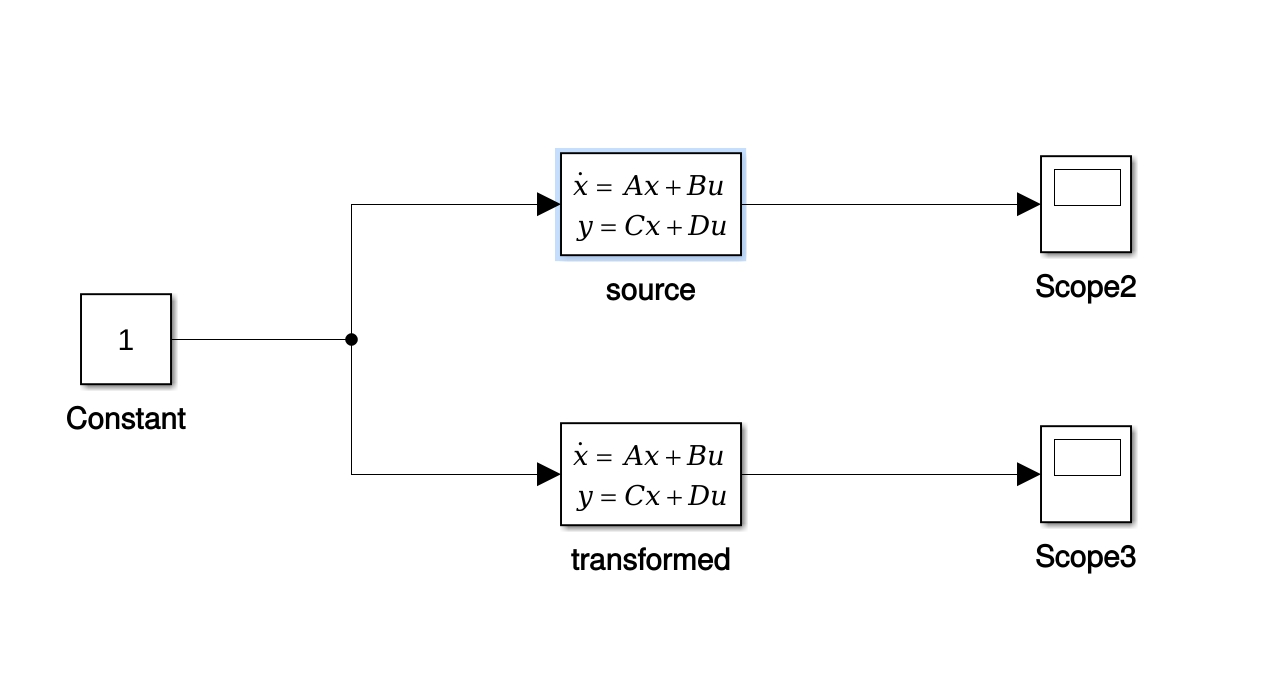
\includegraphics[scale=0.20]{Transform}
		\caption{схема моделирования $u(t) = 1$} 
		\label{pic:pic_5} % название для ссылок внутри кода
	\end{center}
\end{figure}

\begin{figure}[H]
	\begin{center}
		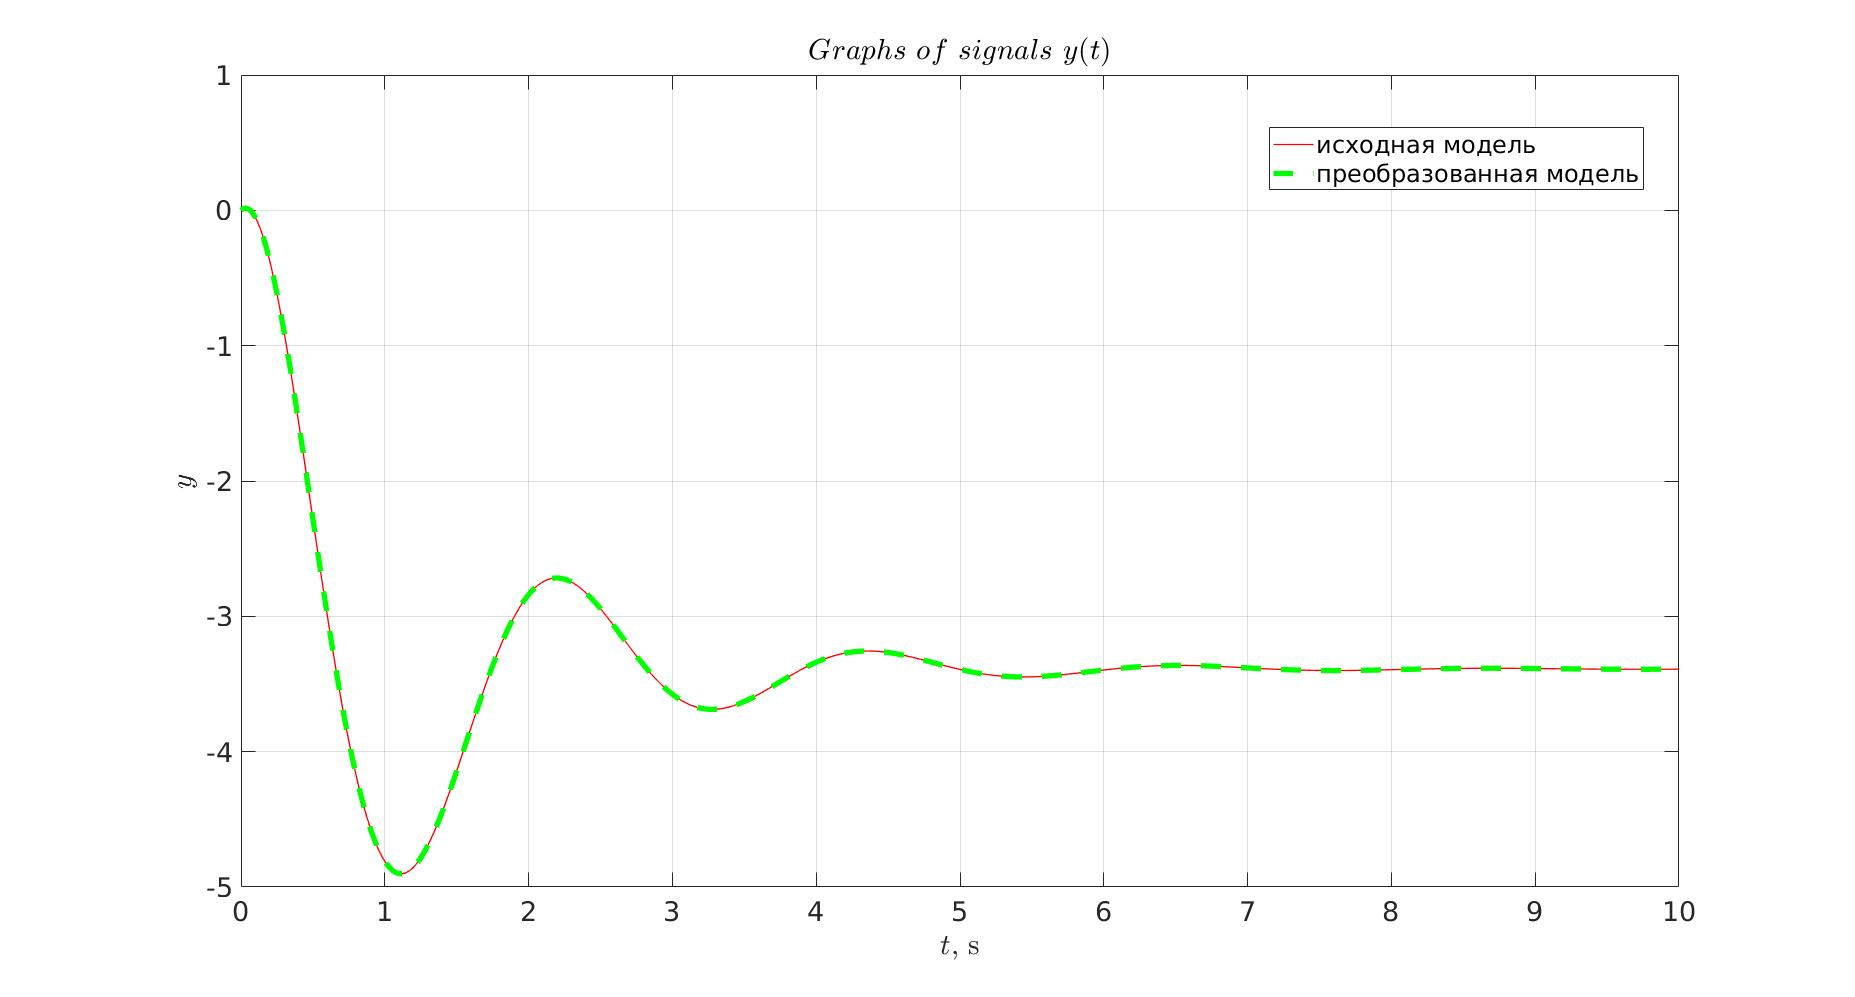
\includegraphics[scale=0.24]{part3}
		\caption{графики моделирования системы} 
		\label{pic:pic_6} % название для ссылок внутри кода
	\end{center}
\end{figure}

\newpage

\section{Вывод}
В данной лабораторной работе были приобретены навыки преобразования системы вход-выход в вход-состояние-выход и обратно. Также были получены навыки представления системы вход-состояние-выход в канонических формах. Одинаковые сигналы с графиков \ref{pic:pic_2} и \ref{pic:pic_4} говорят о том, что были правильно произведены математические преобразования над системами. Также было осуществлено преобразования вектора состояния, а одинаковые сигналы на графиках \ref{pic:pic_6} говрят о том, что все математические дейсвтия верны.
\end{document}
